% Balok dengan rusuk tersembunyi digambar putus-putus
% Konvensi gambar sekolah: 9 rusuk terlihat (garis penuh),
% 3 rusuk tertutup sisi depan (garis putus-putus merah).
% Sisi depan: A(0,0) B(5,0) C(5,3) D(0,3); sisi belakang
% digeser vektor (1,5; 1,2) menjadi E, F, G, H.
\documentclass[tikz,border=8pt]{standalone}
\usepackage{tikz}
\definecolor{navy}{HTML}{14213D}
\definecolor{gold}{HTML}{C9A227}
\begin{document}
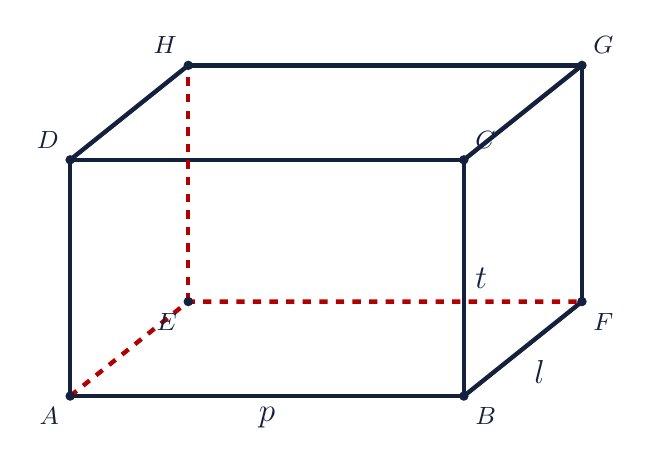
\begin{tikzpicture}[line width=1.6pt, color=navy, x=1cm, y=1cm]
  % Titik sudut sisi depan dan sisi belakang
  \coordinate (A) at (0,0);
  \coordinate (B) at (5,0);
  \coordinate (C) at (5,3);
  \coordinate (D) at (0,3);
  \coordinate (E) at (1.5,1.2);
  \coordinate (F) at (6.5,1.2);
  \coordinate (G) at (6.5,4.2);
  \coordinate (H) at (1.5,4.2);

  % Sisi depan: seluruhnya terlihat
  \draw (A) -- (B) -- (C) -- (D) -- cycle;
  % Rusuk penghubung yang terlihat
  \draw (B) -- (F);
  \draw (C) -- (G);
  \draw (D) -- (H);
  % Sisi belakang: rusuk atas dan kanan terlihat
  \draw (H) -- (G) -- (F);
  % Tiga rusuk tersembunyi: putus-putus
  \draw[dashed, red!70!black] (A) -- (E) -- (F);
  \draw[dashed, red!70!black] (E) -- (H);

  % Label titik sudut
  \foreach \p/\pos in {A/below left, B/below right, C/above right,
    D/above left, E/below left, F/below right, G/above right, H/above left} {
    \fill[navy] (\p) circle (0.06);
    \node[font=\small, \pos] at (\p) {$\p$};
  }
  % Label ukuran: p (panjang), t (tinggi), l (lebar)
  \node[font=\large, below] at (2.5,0) {$p$};
  \node[font=\large, right] at (5,1.5) {$t$};
  \node[font=\large, below right] at (5.75,0.6) {$l$};
\end{tikzpicture}
\end{document}
